\chapter{Caso práctico: Prediciendo propinas en los taxis de Nueva York} \label{chap:5}

\vspace*{5mm}

\section{Introducción} \label{sec:5.1}

A la hora de poner en práctica el conocimiento y el \emph{know-how} obtenidos durante el estudio de los libros [\citeauthor{richert2013building}, ~\citeyear{richert2013building}] y [\citeauthor{abu2012learning}, ~\citeyear{abu2012learning}] (contando además con [\citeauthor{russell2003artificial}, ~\citeyear{russell2003artificial}] para algunos detalles en los algoritmos), tenía que buscar un dataset que satisficiera más mi curiosidad que uno de los que se usa habitualmente de ejemplo, como el famoso \emph{iris}, o de los ya trabajados que podemos encontrar en repositorios como el de la \emph{University of California, Irvine}\footnote{A fecha de entrega de este documento se pueden contar 295 datasets en \url{http://archive.ics.uci.edu/ml/}}.

\begin{figure}[ht]
  \centering
  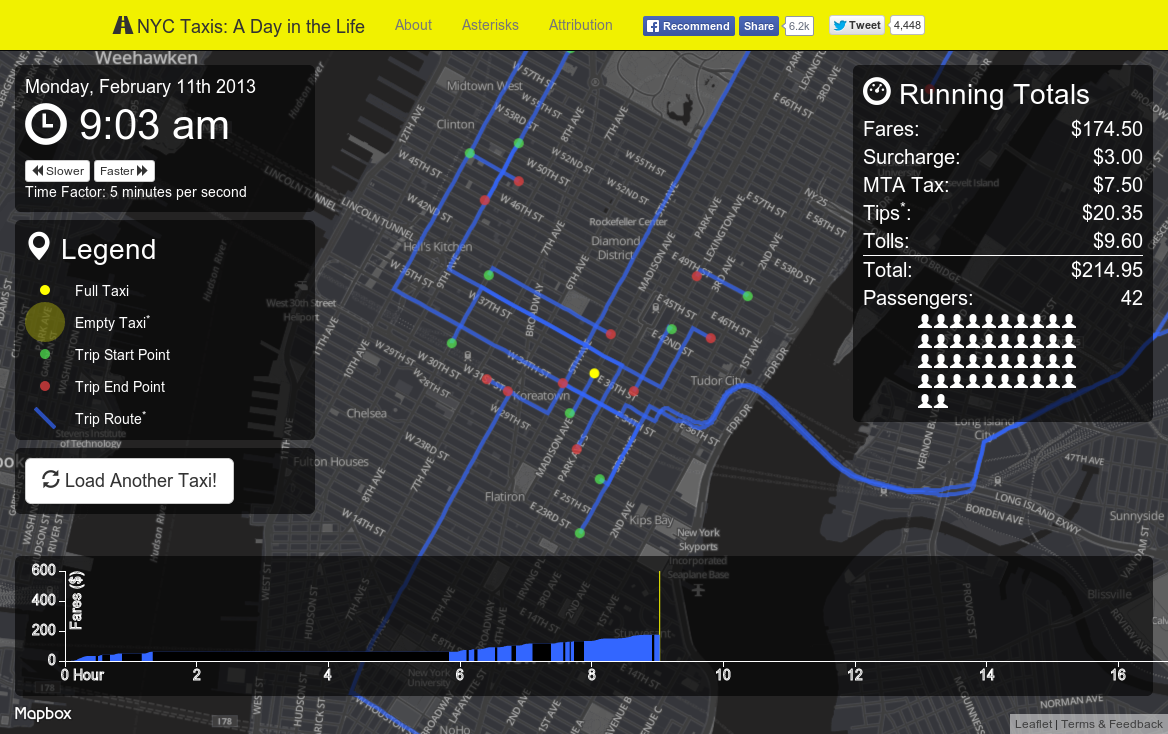
\includegraphics[width=140mm]{figures/ch_05/nyc_taxis_a_day_in_the_life.png}
  \caption{\emph{NYC Taxis: A Day in the Life} monstrando el recorrido de un taxi.}
  \label{fig:5.1}
\end{figure}

El dataset oportuno llegó en la ronda diaria habitual a las noticias relacionadas con tecnología, cuando encontré la web \emph{NYC Taxis: A Day in the Life}\footnote{\url{http://nyctaxi.herokuapp.com/}}. Este sitio mostraba el recorrido de cierto taxi, escogido al azar, de la ciudad de Nueva York durante un día cualquiera de 2013. Además del recorrido, la web mostraba hora, tarifa, propina, número de pasajeros y algún dato importante más sobre cada carrera del taxi, todo en una impresionante visualización de un mapa de Nueva York (figura \ref{fig:5.1}). La primera pregunta que me hice al verlo fue, ¿dónde están esos maravillosos datos?

Chris Whong\footnote{Más información del autor en su blog personal: \url{http://chriswhong.com/}}, el autor de dicha web, fue el que obtuvo esos de datos de la \emph{Comisión de Taxis y Limusinas de la Ciudad de Nueva York}, \emph{NYC Taxi and Limousine Commission} en inglés, de forma bastante manual\footnote{Entrada de su blog donde cuenta su periplo, además de ofrecer enlaces para descargar el dataset: \url{http://chriswhong.com/open-data/foil_nyc_taxi/}}, !tuvo que comprar un disco duro portátil completamente nuevo y entregárselo a esta comisión para que se lo devolvieron con los datos! Así que enhorabuena y muchas gracias por tu trabajo Chris.

El dataset, un total de $48.6GB$ en formato \emph{CSV} al que llamó \emph{nyc\_taxi\_2013}, ofrece los datos de 173.179.759 carreras, $|\mathcal{D}|$, en 24 archivos, utilizando 2 archivos por cada mes del año 2013. Uno de esos dos archivos contiene datos \emph{físicos} de la carrera, como las coordenadas de subida y bajada de pasajeros, hora de inicio y fin de la carrera y distancia recorrida entre otros atributos. El otro abarca la información de la tarifa de la carrera, datos como el precio base, impuestos, peajes y propinas.

En el conjunto de atributos del que se dispone, el más interesante para intentar predecirlo puede ser la \emph{propina}, dada su naturaleza en algunos lugares, ya que en países como Estados Unidos o Canadá, la propina es parte indispensable del sueldo de ciertos trabajadores, por lo que puede interpretarse como un llamamiento al buen trabajo para recibir una mayor propina. Incluso para cada tipo de trabajo existen normas sobre cuánta propina dar, casi siempre basada en porcentajes del cargo total. Así que la pregunta sería, ¿se podrán predecir las propinas en los taxis de Nueva York?

Un maravilloso dataset pero con un gran trabajo por delante, y un gran riesgo de no obtener nada, ya que son datos completamente reales y la cantidad de ruido puede ser muy elevada. Además, puede que los atributos que se tienen no sean los adecuados para esta tarea, por lo que es una apuesta muy arriesgada, pero que si sale bien, puede dar buenos frutos. 

\section{Preparación del dataset} \label{sec:5.2}

Un dataset enorme de datos reales donde el comportamiento humano está involucrado en su construcción puede presentar una tremenda cantidad de ruido, sobre todo en fallos en la anotación de esos datos. Por esa razón este dataset necesita una gran limpieza, donde se eliminarán algunos atributos y muchísimas instancias, y a su vez, nuevos atributos serán creados utilizando el \emph{know-how} adquirido. Durante esta limpieza, podremos determinar cuáles de los atributos que veremos pertenecerán al espacio de entrada, $\mathcal{X}$, y cuales al de salida, $\mathcal{Y}$.

Una vez limpio el dataset, necesitaremos tomar una muestra de él para el aprendizaje, ya que aprender del conjunto completo utilizando las herramientas habituales es una tarea demasiado complicada para poder realizarla.

Al estar los datos divididos en meses, usaremos solo uno de ellos para limpiarlo, y así aprender a automatizar el proceso para aplicarlo al resto de meses. El mes con menos carreras, y por tanto con el que menos vamos a tardar mientras \emph{jugamos} es agosto, con $|\mathcal{D}_{agosto}|\:=$ 12.597.109 carreras.

\subsection{Limpieza de tarifas} \label{subsec:5.2.1}

Empezando con el archivo que contiene la información de la tarifa de cada carrera, primero observaremos su lista de atributos, para después hacer un recorrido por algunos de ellos y ver cómo están distribuidos por las instancias de $\mathcal{D}_{agosto}$.

\begin{description}
\item[medallion] Resumen, \emph{hash}, del número del taxi.

\item[hack\_license] Resumen del número de licencia del taxista.

\item[vendor\_id] Identificador de la marca del sistema de monitorización de carreras.

\item[pickup\_datetime] Fecha y hora de recogida de los pasajeros.

\item[payment\_type] Tipo de pago: tarjeta, efectivo y distintos cheques.

\item[fare\_amount] Tarifa en dólares estadounidenses, como las demás cantidades.

\item[surcharge] Recargo condicionado al trayecto.

\item[mta\_tax] Impuestos.

\item[tip\_amount] Propina.

\item[tolls\_amount] Peajes.

\item[total\_amount] Total pagado.
\end{description}

\begin{figure}[H]
  \centering
  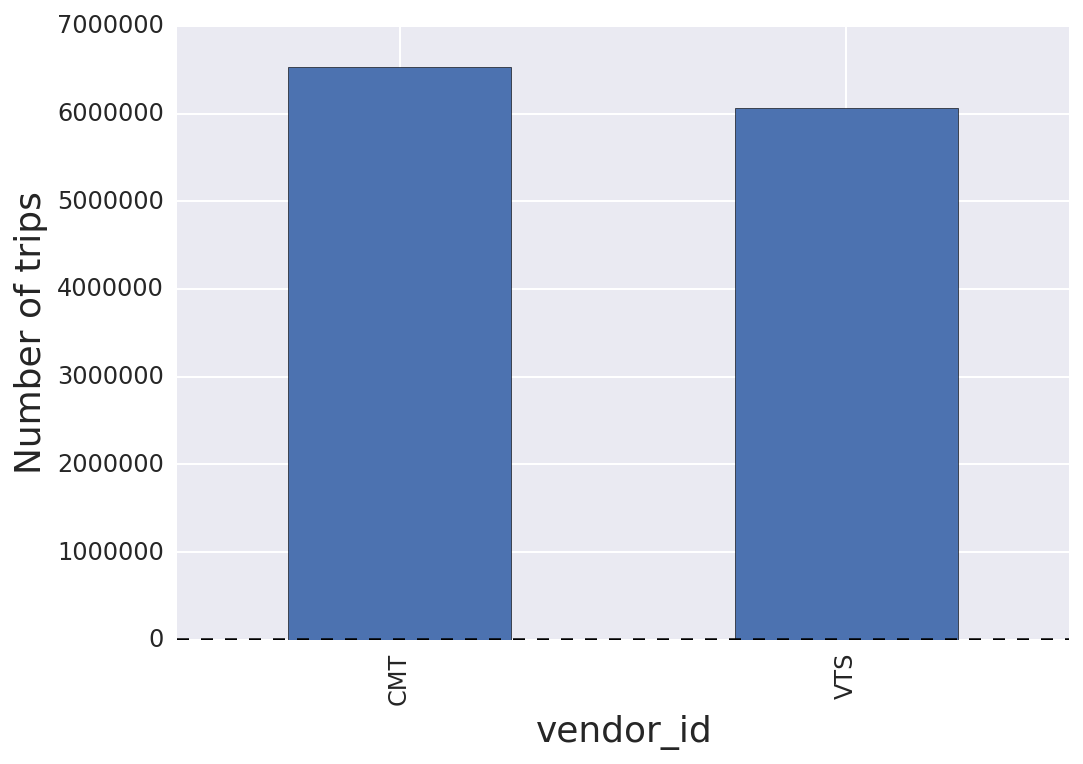
\includegraphics[width=100mm]{figures/ch_05/vendor_id.png}
  \caption{Representación del atributo \emph{vendor\_id} para el mes de agosto.}
  \label{fig:5.2}
\end{figure}

De los cuatro primeros, solo se debería verificar el estado del tercer atributo, \emph{vendor\_id}, así como del quinto en adelante. Si observamos \emph{vendor\_id} en la figura \ref{fig:5.2}, vemos que los valores parecen casi igualmente distribuidos, así que no tenemos que tratarlo.

Si estudiamos el tipo de pago, \emph{payment\_type}, nos encontramos con la figura \ref{fig:5.3}. Aquí podemos eliminar las instancias que no fueron pagadas con tarjeta, \emph{CRD} o en efectivo \emph{CSH}, ya que el número del resto es despreciable.

\begin{figure}[H]
  \centering
  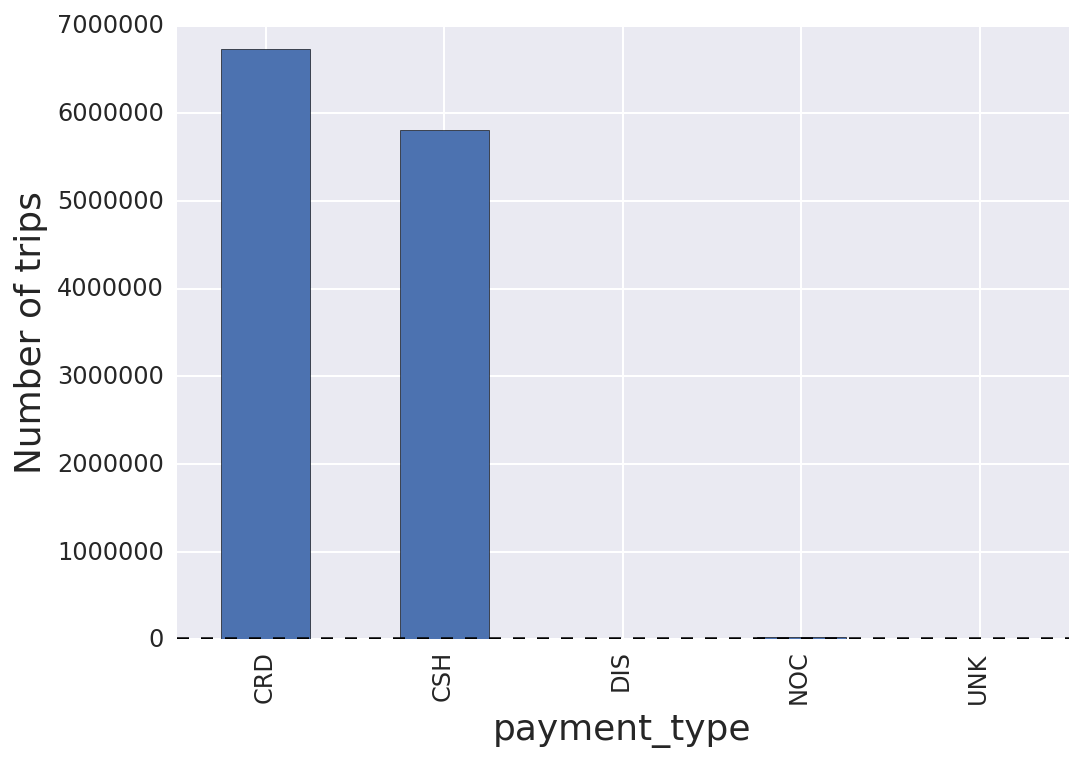
\includegraphics[width=100mm]{figures/ch_05/payment_type_1.png}
  \caption{Representación del atributo \emph{payment\_type} para el mes de agosto.}
  \label{fig:5.3}
\end{figure}

Se puede pensar que con este ajuste, y más aún con los que se harán más adelante, se está \emph{sesgando} el dataset, haciendo que también esté sesgado el aprendizaje y lo que puede predecir. Y así es, aunque en este caso esto no debería ser un problema, ya que lo que vamos a predecir son instancias igualmente sesgadas. Además, estos ajustes \emph{a conveniencia} son mínimos, ya que la gran mayoría de los que se hagan más adelante, se harán para eliminar ciertos problemas, que van desde errores en las medidas de ciertos instrumentos, como por ejemplo coordenadas que no existen en el globo terráqueo o carreras que duran \emph{millones} de millas; errores al introducir cantidades, como por ejemplo cientos de miles de dólares como total pagado en efectivo en una carrera; o casos para nada ordinarios, como carreras que duran varias horas.

\begin{table}[ht]
\centering
\colorbox{lightgray}{\begin{tabular}{*{4}{c}}
  & \emph{\textbf{fare\_amount}} & \emph{\textbf{tip\_amount}} & \emph{\textbf{tolls\_amount}} \\
  $\mathbf{\bar{x}}$ & $12.57$ & $1.36$ & $0.28$ \\
  $\mathbf{\sigma}$ & $54.54$ & $2.35$ & $1.50$ \\
  \textbf{min} & $-1430.00$ & $-96.82$ & $-22.25$ \\
  $\mathbf{Q_{1}}$ & $6.50$ & $0.00$ & $0.00$ \\
  $\mathbf{Q_{2}}$ & $9.50$ & $1.00$ & $0.00$ \\
  $\mathbf{Q_{3}}$ & $14.00$ & $2.00$ & $0.00$ \\
  \textbf{max} & $158995.81$ & $888.19$ & $960.09$
\end{tabular}}
\caption{Representación de los atributos \emph{fare\_amount}, \emph{tip\_amount} y \emph{tolls\_amount} para el mes de agosto.}
\label{table:5.1}
\end{table}

Sigamos analizando atributos. El atributo de la tarifa, \emph{fare\_amount}, no tiene fácil visualización, así que nos fijaremos en la tabla \ref{table:5.1}, donde representamos ciertas medidas estadísticas. Aquí podemos observar un gran error, como uno de los que se comentó anteriormente: la tarifa mínima ha sido $-1430.00\$$. Observando la tabla y aplicando algo de sentido común, podemos limitar este atributo a valores, por ejemplo, de entre $3.00$ a $200.00$ dólares.

\begin{figure}[H]
  \centering
  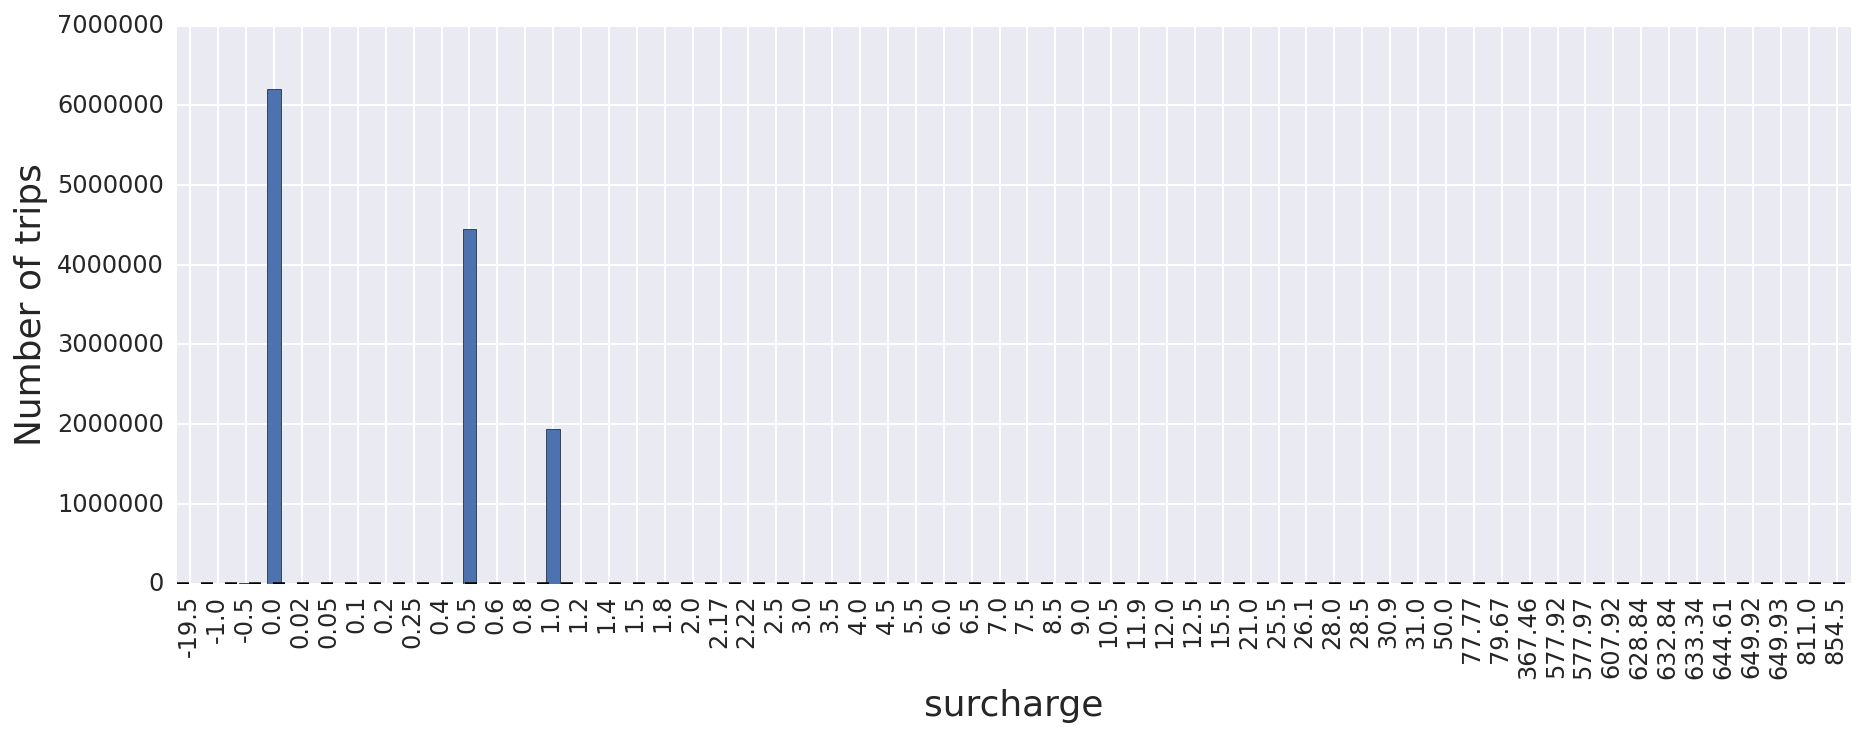
\includegraphics[width=140mm]{figures/ch_05/surcharge.png}
  \caption{Representación del atributo \emph{surcharge} para el mes de agosto.}
  \label{fig:5.4}
\end{figure}

Para el recargo, \emph{surcharge}, vemos que en la figura \ref{fig:5.4} solo hay tres valores importantes $0.00$, $0.50$ y $1.00$ dólar. Así que nos limitaremos a ellos.

\begin{figure}[H]
  \centering
  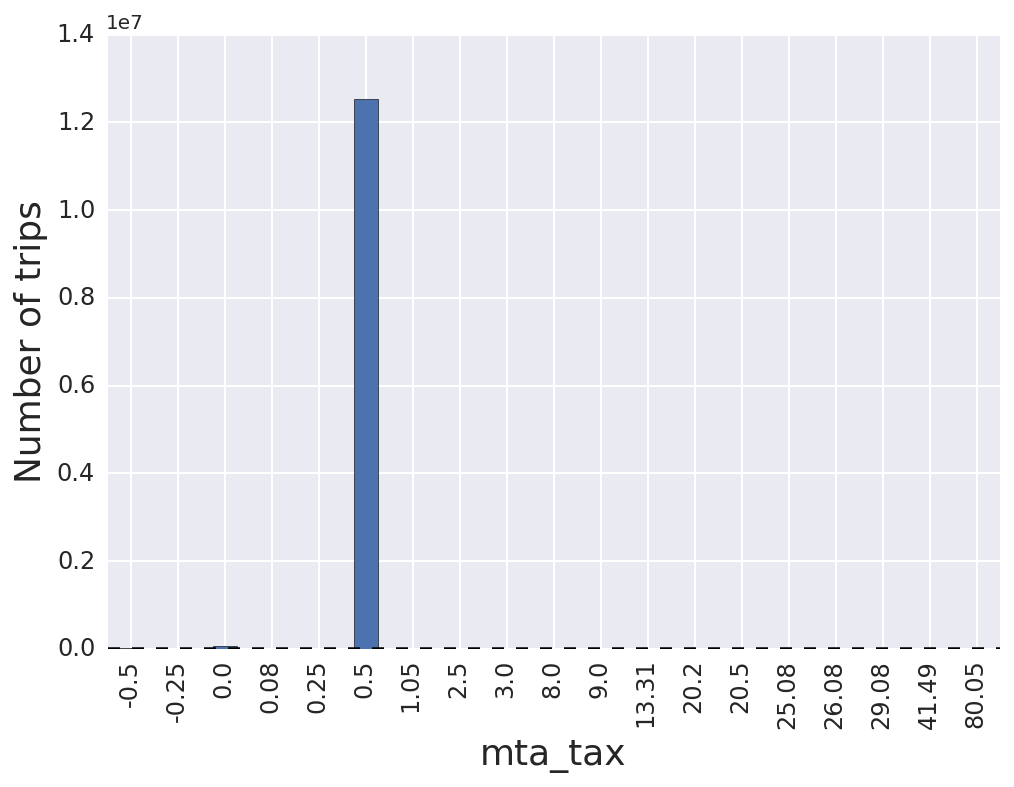
\includegraphics[width=100mm]{figures/ch_05/mta_tax.png}
  \caption{Representación del atributo \emph{mta\_tax} para el mes de agosto.}
  \label{fig:5.5}
\end{figure}

Para los impuestos, \emph{mta\_tax}, vemos en la figura \ref{fig:5.5} cómo prácticamente se limita a un valor, $0.50\$$, el único que se usará. Además al tener únicamente un valor podremos eliminar dicha variable del dataset.

Con el atributo de las propinas, \emph{tip\_amount}, tenemos el mismo problema que en la tarifa, así que lo representamos en la tabla \ref{table:5.1}. Volviéndonos a encontrar con valores negativos, tenemos que sesgar las instancias dependiendo de ciertos valores para la propina. Parecido a lo se hizo en la tarifa, podemos eliminar aquellas instancias cuya propina no esté entre $0.00$ y $100.00$ dólares, valores algo más ordinarios. Como hemos comentado, este atributo será el que queremos predecir.

También tenemos el mismo problema con los peajes, \emph{tolls\_amount} como vemos en la tabla \ref{table:5.1}. Además, como estos cambian conforme el transcurso del año se hace difícil buscar valores fijos para limitar las instancias. Si obtenemos cuáles son los valores que se repiten más de $1000$ veces, estos van desde $0.00$ a un máximo de $15.58$ dólares. Así, podemos pensar que un buen sesgo podría ser limitar el peaje a valores entre $0.00$ y $30.00$ dólares.

En \emph{total\_amount} no nos fijaremos, ya que es la suma total de las cantidades anteriores, que están corregidas. Cualquier error en ese atributo será bastante improbable, pudiendo ser casi exclusivamente modificaciones a mano, algo que nos nos importa ya que no usaremos esta variable durante el aprendizaje, porque al unirla con las anteriores hace que tengamos implícitamente el valor la propina disponible.

\begin{figure}[ht]
  \centering
  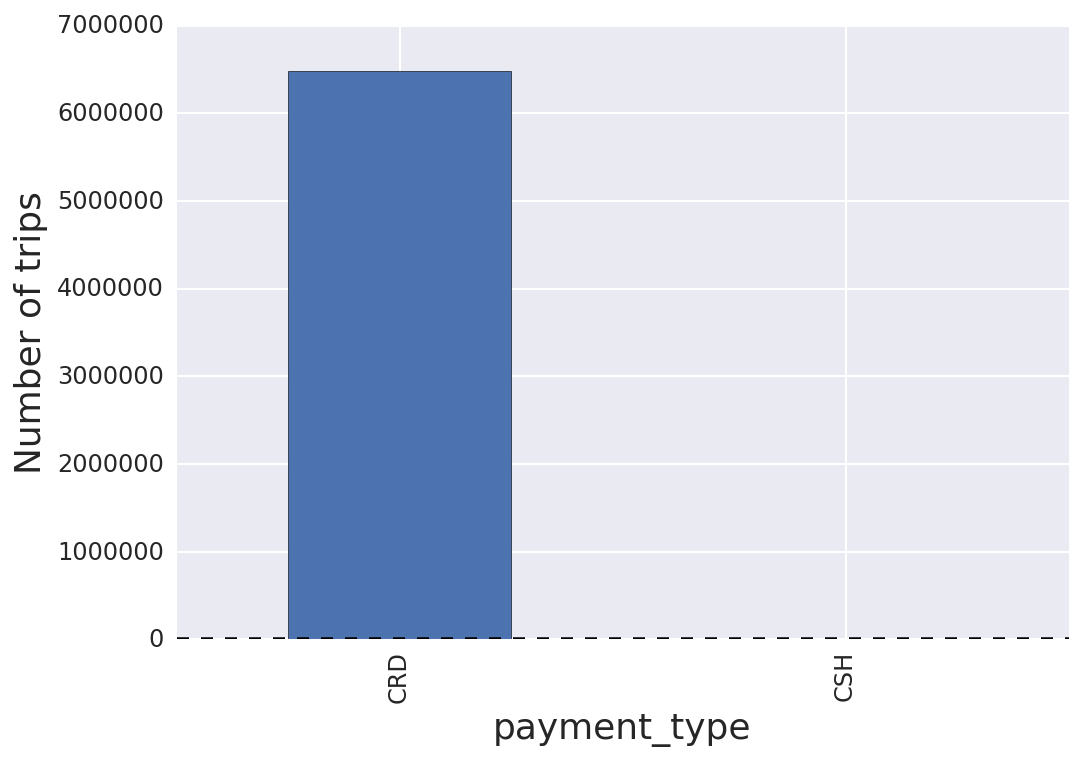
\includegraphics[width=100mm]{figures/ch_05/payment_type_2.png}
  \caption{Representación del atributo \emph{payment\_type} para propinas mayores de $0.00\$$ en el mes de agosto.}
  \label{fig:5.6}
\end{figure}

Antes de acabar con este archivo y empezar a analizar el archivo con las propiedades físicas de las carreras, vamos a realizar dos cosas, saciar mi curiosidad y crear un nuevo atributo. Sentía gran curiosidad de saber si los taxistas registran las propinas cuando sus clientes les pagan en efectivo. Y como podemos observar en la figura \ref{fig:5.6} la realidad es que no. La cantidad es tan ínfima que no es observable en la figura, y por esta razón se pueden limitar las instancias a sólo las pagadas con tarjeta, pudiendo eliminar esta variable al tener nada más que un valor.

Sobre el nuevo atributo que se comentó antes, será uno que hará más fácil el aprendizaje de las propinas: el porcentaje de propina de la carrera, al que llamaremos \emph{tip\_perc}. Para ellos usaremos la siguiente función:

$$
tip\_perc\:=\:\frac{tip\_amount}{fare\_amount\:+\:surcharge\:+\:mta\_tax}\:\cdot\:100
$$

\noindent
y además limitaremos las propinas hasta un máximo del $50\%$ para descartar valores muy atípicos. Así, para el aprendizaje y la predicción podemos sustituir la variable \emph{tip\_amount} por esta nueva, que posee valores totalmente normalizados para todas las carreras.

\subsection{Limpieza del resto de información} \label{subsec:5.2.2}

Para limpiar el segundo y último archivo, el que contiene la información física de las carreras, vamos a echar un vistazo a la información que contiene por cada carrera, para después, como con el archivo anterior, pararnos en algunos de ellos para su limpieza.

\begin{description}
\item[medallion] Resumen, \emph{hash}, del número del taxi.

\item[hack\_license] Resumen del número de licencia del taxista.

\item[vendor\_id] Identificador de la marca del sistema de monitorización de carreras.

\item[rate\_code] Código indicando el tipo de carrera.

\item[store\_and\_fwd\_flag] Carrera con destinos múltiples.

\item[pickup\_datetime] Fecha y hora de recogida de los pasajeros.

\item[dropoff\_datetime] Fecha y hora de bajada de los pasajeros.

\item[passenger\_count] Número de pasajeros.

\item[trip\_time\_in\_secs] Duración en segundos.

\item[trip\_distance] Distancia en millas.

\item[pickup\_longitude] Longitud de recogida.

\item[pickup\_latitude] Latitud de recogida.

\item[dropoff\_longitude] Longitud de bajada.

\item[dropoff\_latitude] Latitud de bajada.
\end{description}

Antes de comenzar podemos ver que ciertos atributos del archivo anterior se repiten en este. Al estar cada carrera partida en dos archivos, ¿cómo sabemos que datos son de la misma carrera? Al estar en formato CSV podemos usar el número de linea para identificar las carreras, así que los datos de la línea 19 de cada uno de los dos archivos corresponderían a la misma carrera. Efectivamente esto es así, aunque no se describe en ningún lugar. Para comprobarlo podemos usar los atributos que se repiten a modo de índice, siendo tan sólo realmente necesarios \emph{medallion} o \emph{hack\_license} acompañados de \emph{pickup\_datetime}. Por lo tanto podemos descartar los cuatro atributos repetidos en este archivo.

\begin{figure}[ht]
  \centering
  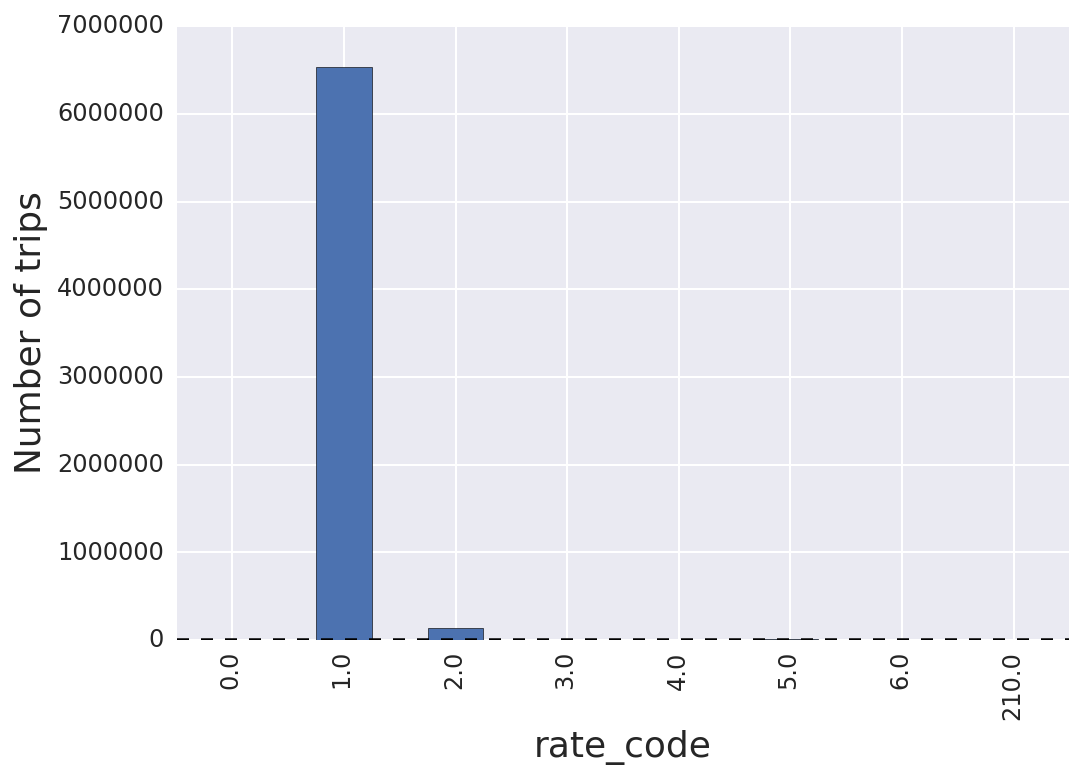
\includegraphics[width=100mm]{figures/ch_05/rate_code.png}
  \caption{Representación del atributo \emph{rate\_code} para el mes de agosto.}
  \label{fig:5.7}
\end{figure}

Empecemos con el primero de los atributos no repetidos, \emph{rate\_code}. Como se puede observar en la figura \ref{fig:5.7}, los valores de este atributo casi se limitan a $1$. Por lo tanto podemos filtrar las instancias a este único valor, y además eliminar la variable al tener un valor único.

Con el siguiente atributo, \emph{store\_and\_fwd\_flag}, existe un problema un poco grave: faltan muchos valores y además no queda claro lo que significan los existentes. Así que eliminaremos este atributo sin poder limpiarlo, dejando un poco de ruido más al existente en el dataset.

Como la fecha y hora de bajada de pasajeros, \emph{dropoff\_datetime}, esta implícita en la duración del trayecto podemos eliminar completamente este atributo.

\begin{figure}[ht]
  \centering
  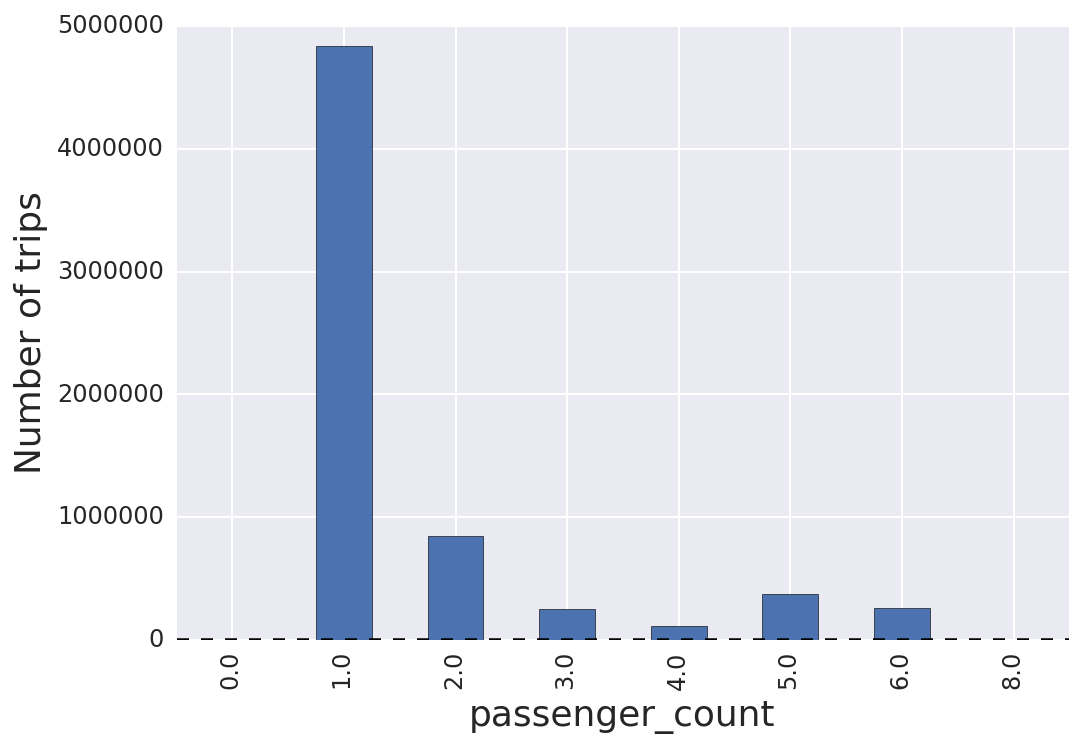
\includegraphics[width=100mm]{figures/ch_05/passenger_count.png}
  \caption{Representación del atributo \emph{passenger\_count} para el mes de agosto.}
  \label{fig:5.8}
\end{figure}

Para limpiar el número de pasajeros, \emph{passenger\_count}, veamos la figura \ref{fig:5.8}. En ella podemos observar que los valores destacables del número de pasajeros van de $1$ a $6$, así que el resto se eliminarán.

\begin{table}[H]
\centering
\colorbox{lightgray}{\begin{tabular}{*{3}{c}}
  & \emph{\textbf{trip\_time\_in\_secs}} & \emph{\textbf{trip\_distance}} \\
  $\mathbf{\bar{x}}$ & $1435.24$ & $82.36$ \\
  $\mathbf{\sigma}$ & $52463.44$ & $25494.24$ \\
  \textbf{min} & $-10.00$ & $0.00$ \\
  $\mathbf{Q_{1}}$ & $420.00$ & $1.19$ \\
  $\mathbf{Q_{2}}$ & $660.00$ & $2.00$ \\
  $\mathbf{Q_{3}}$ & $1020.00$ & $3.63$ \\
  \textbf{max} & $4294966.00$ & $15038005.00$
\end{tabular}}
\caption{Representación de los atributos \emph{trip\_time\_in\_secs} y \emph{trip\_distance} para el mes de agosto.}
\label{table:5.2}
\end{table}

Los dos siguientes, \emph{trip\_time\_in\_secs} y \emph{trip\_distance}, tienen difícil representación gráfica, así que observemos la tabla \ref{table:5.2}. De nuevo podemos observar que existen atributos con valores erróneos, como los negativos; o absurdos, como $15\:millones$ de millas. Así que para este par de variables, vamos a medir el tiempo y la distancia que se tardaría en un trayecto bastante largo en la ciudad de Nueva York, por ejemplo el que va desde el \emph{Aeropuerto Internacional John F. Kennedy} al norte del \emph{Bronx}, uno de los cinco distritos de la ciudad, por ejemplo, a la calle 236 oeste. Según \emph{Google Maps} este trayecto con mucho atasco debido al tráfico, dura en torno a los $52$ minutos y recorre una distancia de $22.1$ millas, unos $35.5$ kilómetros. Así que, siendo este un trayecto muy largo, podemos limitar el tiempo del viaje para dejarlo entre $0$ y $3600$ segundos, sin contar con el $0$ exacto. La distancia recorrida podemos dejarla entre $0$ y $25$ millas, de nuevo sin contar con el $0$. Las instancias que no cumplan estas restricciones, serán eliminadas.

\begin{table}[H]
\centering
\colorbox{lightgray}{\begin{tabular}{*{3}{c}}
  & \emph{\textbf{min}} & \emph{\textbf{max}} \\
  \emph{\textbf{latitude}} & $40.459518$ & $41.175342$ \\
  \emph{\textbf{longitude}} & $-74.361107$ & $-71.903083$
\end{tabular}}
\caption{Coordenadas que crean el área de la figura \ref{fig:5.9}.}
\label{table:5.3}
\end{table}

Por último tratemos con las coordenadas. Estas son un verdadero caos, ya que las hay en en el origen de coordenadas, cerca del golfo de Guinea, con valores gigantescos o, aunque cerca de Nueva York, apuntando al mar. Entonces, primero las limitaremos a los valores de la tabla \ref{table:5.3}, resultando en el área de la figura \ref{fig:5.9}, dejando bastante margen al este y al oeste para posibles trayectos en esas zonas.

\begin{figure}[H]
  \centering
  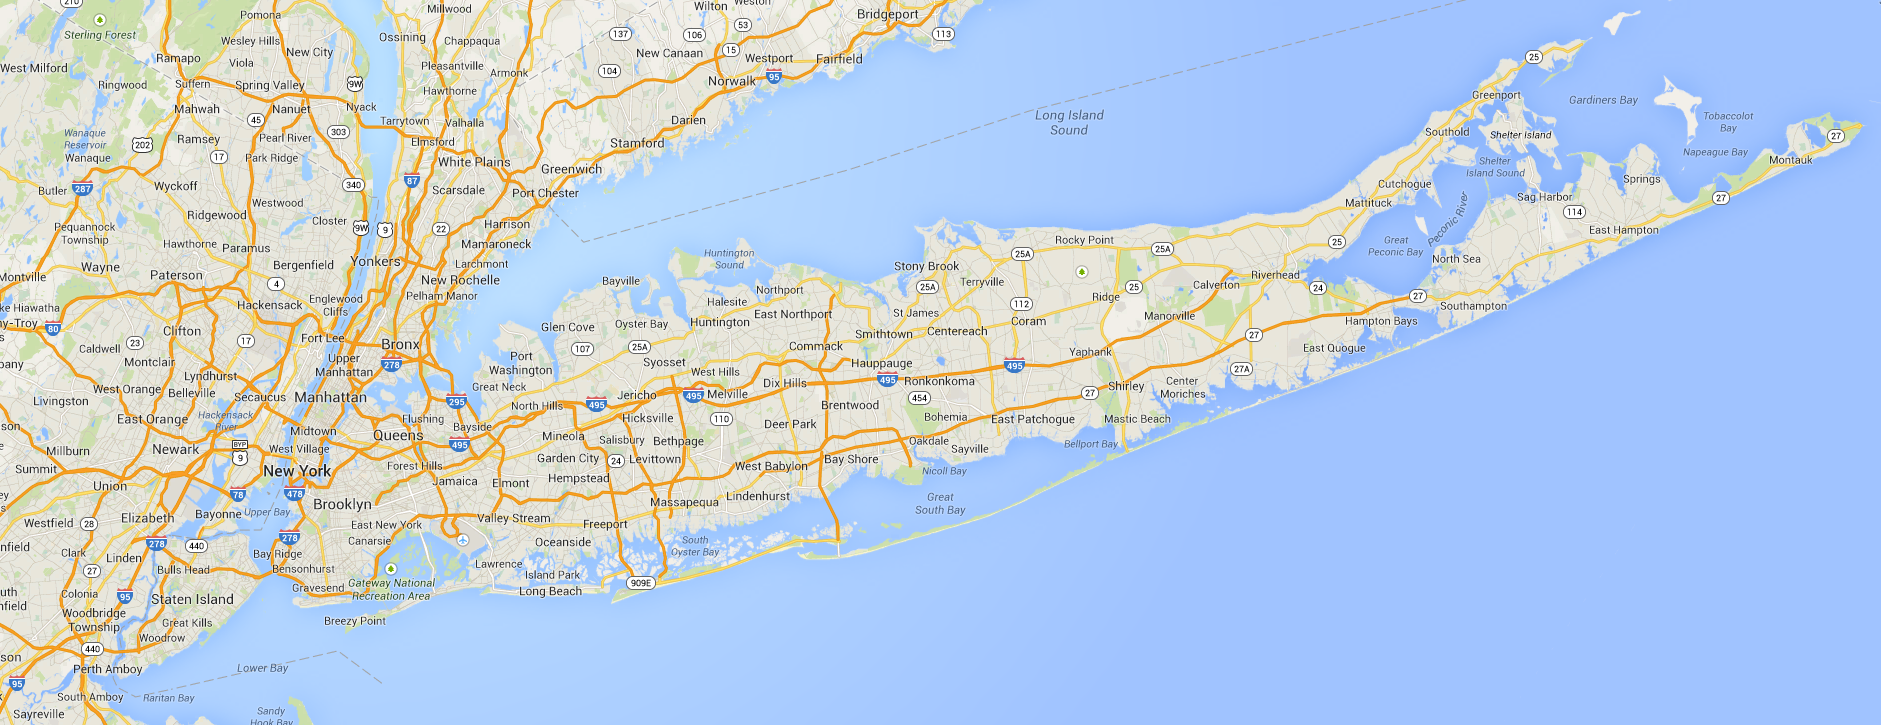
\includegraphics[width=140mm]{figures/ch_05/map_1.png}
  \caption{Mapa del área seleccionada extraído de \href{https://maps.google.com}{\emph{Google Maps}}.}
  \label{fig:5.9}
\end{figure}

Para comprobar que existen coordenadas en el mar solo basta con observar la figura \ref{fig:5.10}, donde vemos un conjunto de coordenadas que representan el suroeste de la ciudad. A parte de las calles, vemos como la gran superficie blanca es la desembocadura del \emph{río Hudson}, donde también se encuentran muchas de las coordenadas de las carreras. 

\begin{figure}[H]
  \centering
  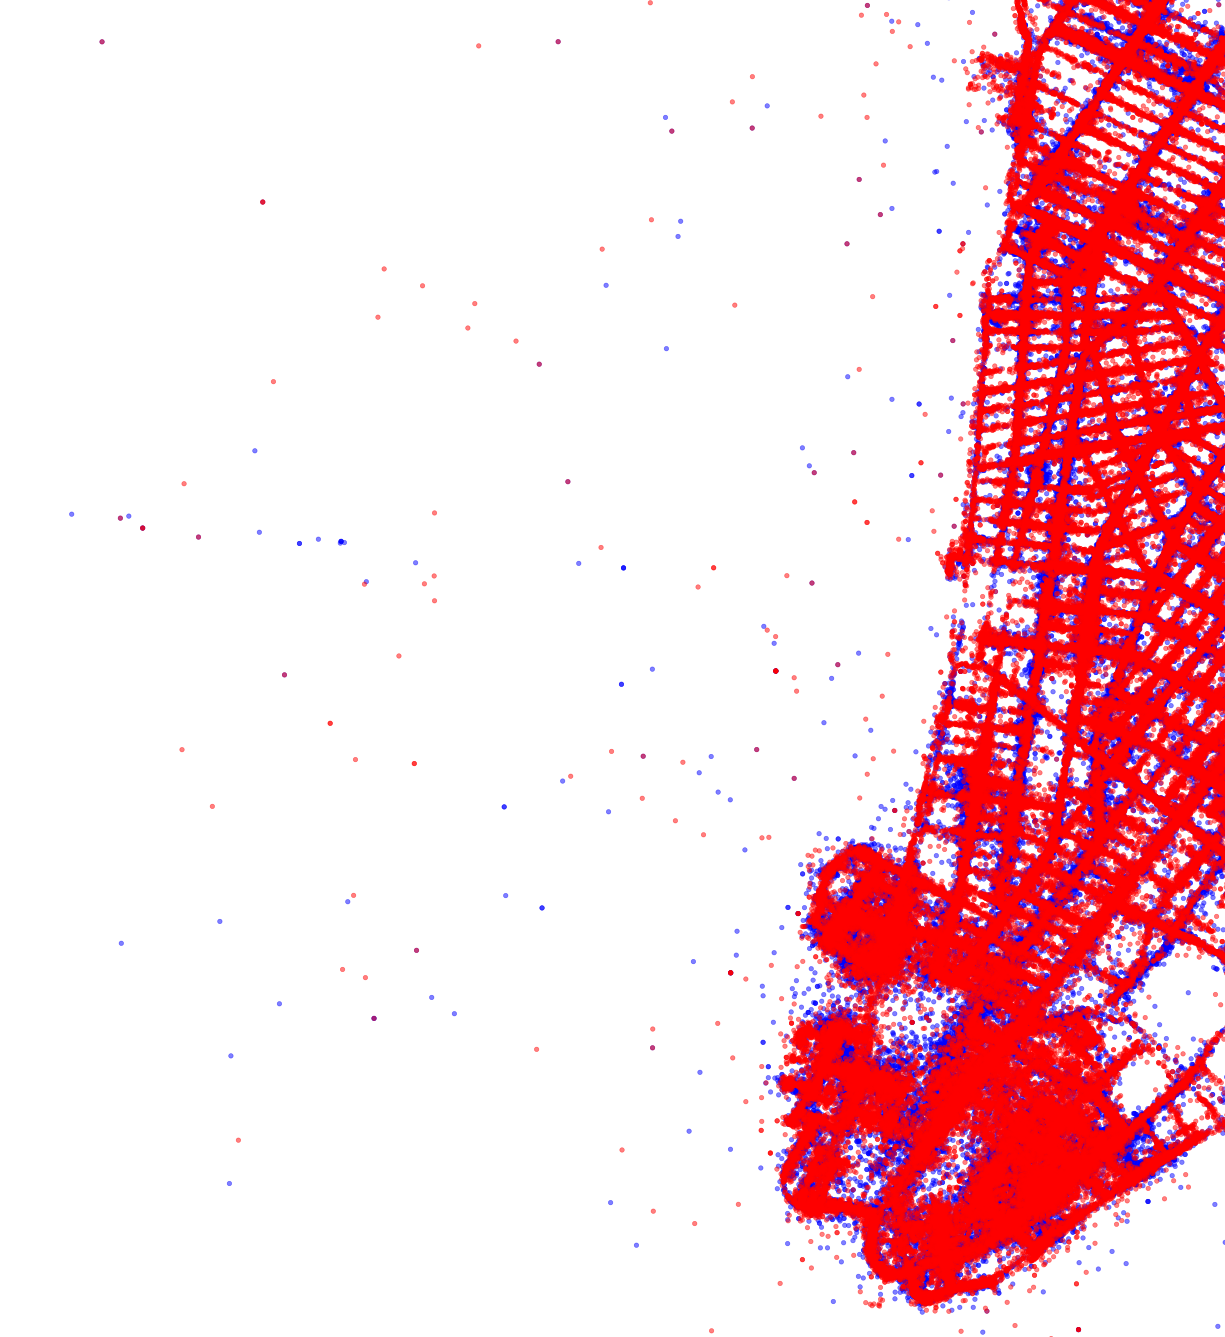
\includegraphics[width=140mm]{figures/ch_05/map_2.png}
  \caption{Representación de las coordenadas donde se observan algunas en el agua. Los puntos azules indican recogidas de pasajeros y los rojos sus posteriores bajadas.}
  \label{fig:5.10}
\end{figure}

Para eliminar bastantes instancias que disponen de este ruido de los dispositivos \emph{GPS} sin recurrir a una lenta herramienta \emph{GIS}, una posible solución es dividir el espacio de coordenadas en \emph{pequeñas} áreas cuadradas, y eliminar las instancias cuyas áreas, recogida y bajada, contengan un número de carreras menor a uno determinado. Por ejemplo, se pueden usar áreas de 270 metros de lado aproximadamente, como se muestra en la figura \ref{fig:5.11}. Como cantidad de carreras a sesgar se podría usar un número variante según la zona, pero para simplificar el problema, se ha optado por $20$.

\begin{figure}[H]
  \centering
  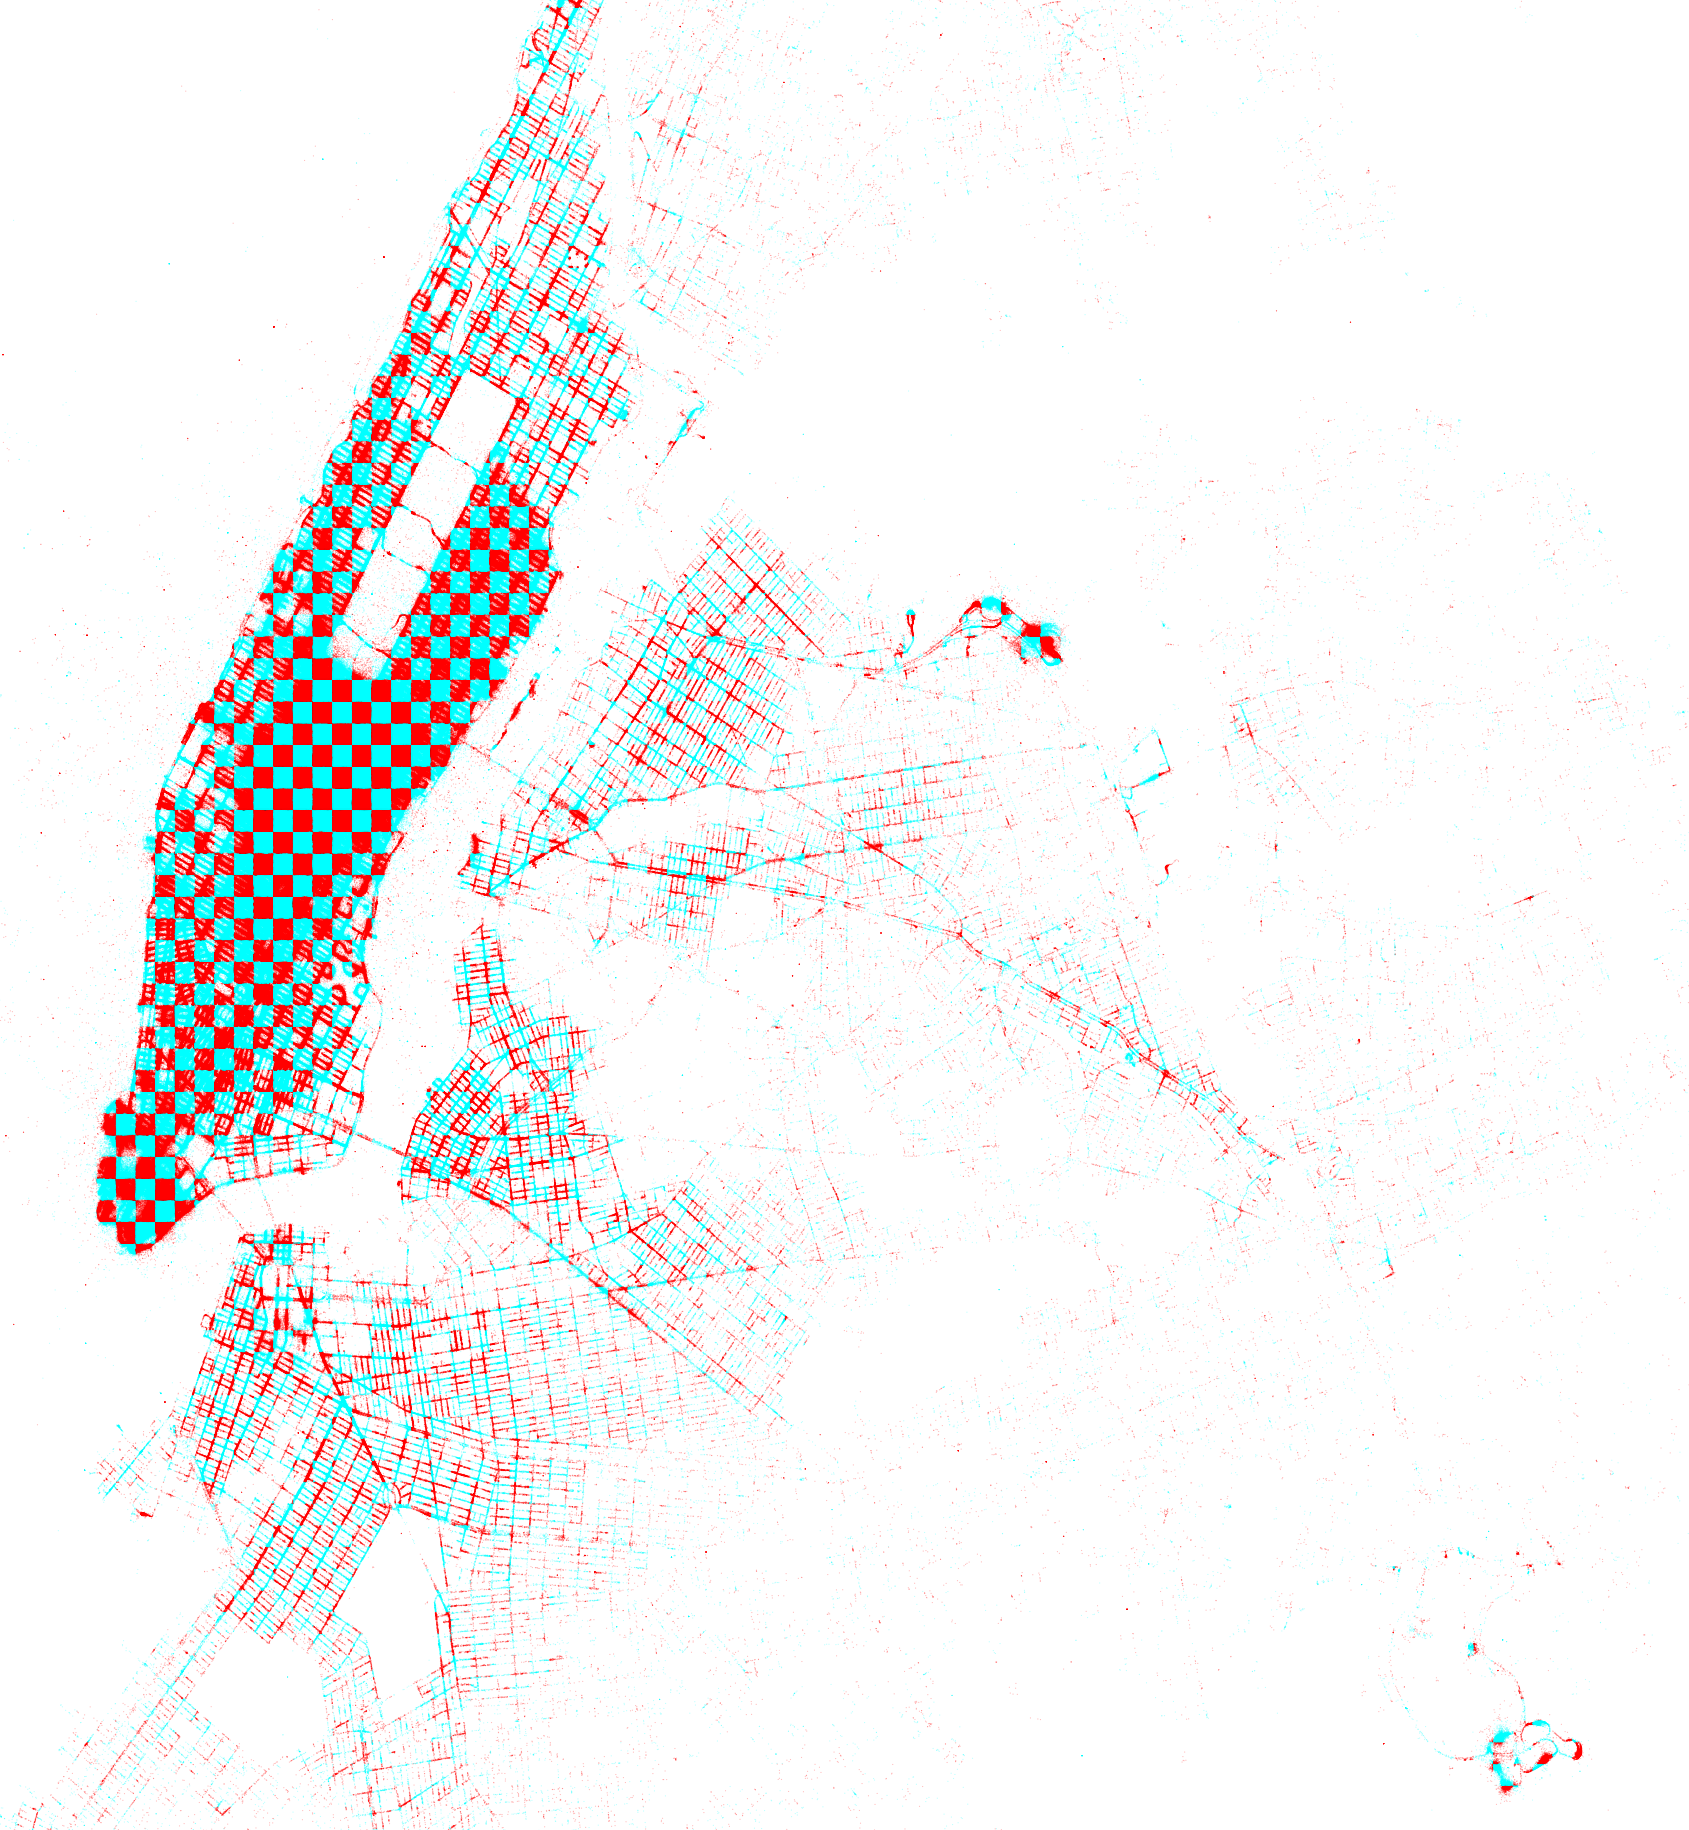
\includegraphics[width=140mm]{figures/ch_05/map_3.png}
  \caption{Representación de las \emph{pequeñas} áreas de coordenadas.}
  \label{fig:5.11}
\end{figure}

Con este último paso podemos finalizar el proceso de limpieza de los datos del mes de agosto. Ahora, tan sólo quedaría crear un pequeño proceso que realice los mismos pasos para el resto de meses, y de esta manera disponer de una versión limpia del dataset al completo.

Una vez que este proceso haya limpiado los más de $170\:millones$ de carreras, en $48.6GB$, se pasará a disponer de 88.156.805 carreras limpias en $17.3GB$, habiéndose eliminado de esta manera el $49.1\%$ de las carreras y el $64.4\%$ del tamaño del dataset.

\subsection{Ajuste del tamaño del dataset} \label{subsec:5.2.3}

Un dataset con más de $88\:millones$ de instancias. Seguramente al aprender de todas ellas nos encontraríamos problemas de sobreajuste, o dependiendo del modelo, con la imposibilidad de usarlas al completo por falta de recursos. Para solucionar este problema crearemos un nuevo dataset a partir de un subconjunto, escogido al azar, de las instancias del original, por ejemplo, de un millón de carreras.

Una vez ajustado el tamaño, es el momento de incluir más atributos en el dataset. Dado que este ha pasado por los filtros de la subsección anterior, no hará falta limpiar los nuevos atributos, y el tamaño del dataset será el mismo. Por ejemplo, podríamos eliminar la variable \emph{pickup\_datetime} para dividirla en atributos numéricos y categóricos con mayor significado en su conjunto. Por ejemplo, la siguiente lista representa una serie de atributos con información del momento en el que se recogieron pasajeros:

\begin{description}
\item[pickup\_month] Mes.

\item[pickup\_weekday] Día de la semana.

\item[pickup\_day] Día del mes.

\item[pickup\_time\_in\_mins] Hora representada en minutos. Por ejemplo, las 16:32 se representaría como $992$.

\item[pickup\_non\_working\_today] Un valor booleano que dice si ese día era laborable.

\item[pickup\_non\_working\_tomorrow] Un valor booleano que dice si el día siguiente era laborable.
\end{description}

Toda la información de esos atributos estaba representada en la variable \emph{pickup\_datetime} (por lo que se puede eliminar) a excepción de las dos últimas, que se ha utilizado información de los días festivos en la ciudad de Nueva York\footnote{NYC holiday calendar: \href{http://www.nyc.gov/html/opa/downloads/pdf/3-year\%20Calendar\%202013-2014-2015.pdf}{http://www.nyc.gov/downloads/3-year-calendar.pdf}}.

Predecir la propina según el porcentaje de ella es una problema de regresión. Generalmente, la regresión ofrece peores resultados cuando existen problemas de ruido, sobre todo cuando es \emph{ruido humano}, como en este caso. Para ello, eliminaremos esa variable y crearemos otra nueva, \emph{tip\_label}, convirtiendo el problema en uno de clasificación. Conociendo de antemano que el porcentaje de propinas puede ir de $0$ a $50$, ambos incluidos, unas buenas etiquetas pueden ser las siguientes:

$$
[0,\:10),\:[10,\:15),\:[15,\:20),\:[20,\:25),\:[25,\:30)\:y\:[30,\:+\infty)
$$

\noindent

quedando las instancias distribuidas según la figura \ref{fig:5.12}.

\begin{figure}[ht]
  \centering
  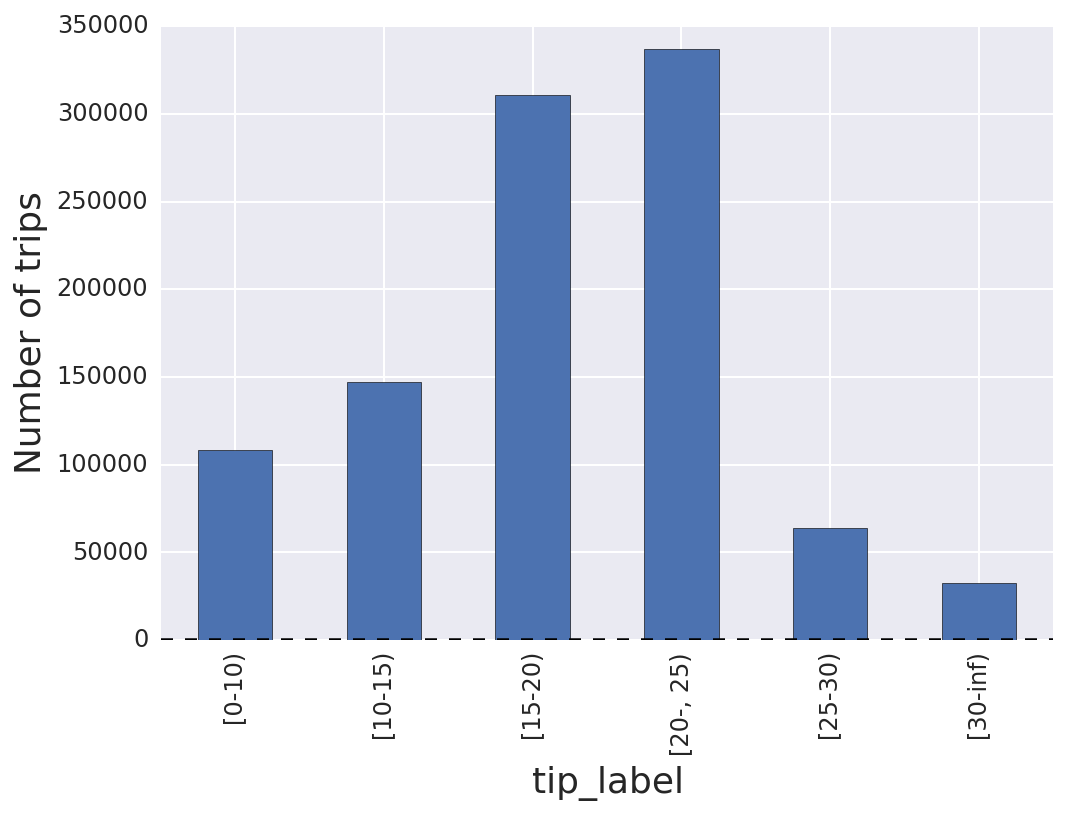
\includegraphics[width=100mm]{figures/ch_05/tip_label_1.png}
  \caption{Representación del atributo \emph{tip\_label}.}
  \label{fig:5.12}
\end{figure}

\pagebreak

Una vez realizadas estas tareas tenemos listos los datos para su aprendizaje. Como breve repaso, el dataset ha quedado de la siguiente manera:

\vspace*{-5mm}

\begin{itemize}
\item[\textbullet]$|\mathcal{D}|\:=\:$1.000.000

\item[\textbullet]$\mathcal{X}\:=\:[$\emph{medallion}, \emph{hack\_license}, \emph{vendor\_id}, \emph{pickup\_month}, \emph{pickup\_weekday}, \emph{pickup\_day}, \emph{pickup\_time\_in\_mins}, \emph{pickup\_non\_working\_today}, \emph{pickup\_non-\_working\_tomorrow}, \emph{fare\_amount}, \emph{surcharge}, \emph{tolls\_amount}, \emph{passenger\_count}, \emph{trip\_time\_in\_secs}, \emph{trip\_distance}, \emph{pickup\_longitude}, \emph{pickup\_latitude}, \emph{dropoff-\_longitude}, \emph{dropoff\_latitude}$]$

\item[\textbullet]$\mathcal{Y}\:=\:[$\emph{tip\_label}$]$
\end{itemize}

\vspace*{5mm}

\section{Aprendizaje y medida del rendimiento} \label{sec:5.3}

A la hora de aprender, aparte de los datos, necesitamos un algoritmo. Dada mi poca experiencia, sobre todo en la parte teórica, no sabía qué modelo escoger para ello, un indicador de hacia dónde deben continuar mi estudios sobre machine learning. Para solucionar esto le pregunté a Fernando, mi director de proyecto, sobre una recomendación. Su elección fué bastante clara, dada su experiencia en otros proyectos relacionados con machine lerning: \emph{random forest}. Este método, una combinación de árboles de decisión tal como se vió en la subsección \ref{subsec:3.1.4}, se ha popularizado bastante en la red desde hace un par de años. La razón para esto es que actualmente se disponen de máquinas con los recursos necesarios para mantener uno de estos \emph{bosques} en memoria, y así poder operar con él de manera más eficiente que en disco.

El aprendizaje se configuró para que se usara \emph{validación cruzada} con \emph{$10$-fold} y \emph{estratificación}, para crear \emph{$256$ árboles}, una bonita potencia de $2$, en cada iteración.

Los resultados no fueron buenos, tan sólo un $52.95\%$ de exactitud. Las causas de esto podían ser múltiples y complejas. Por suerte, observé la matriz de confusión obtenida durante la validación, que se muestra en la figura \ref{fig:5.13}.

\begin{figure}[H]
  \centering
  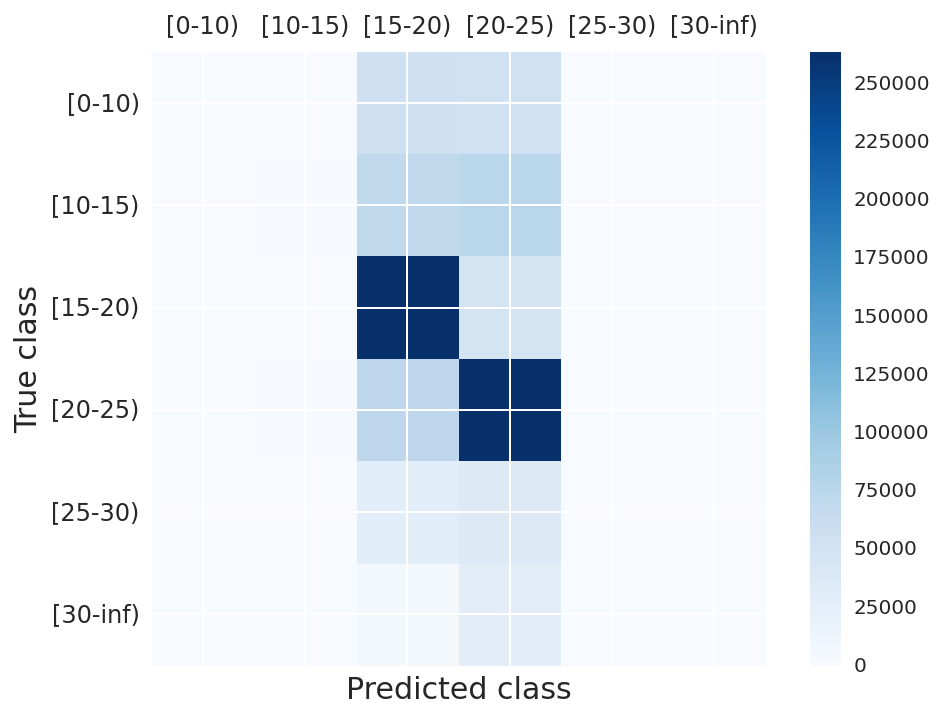
\includegraphics[width=100mm]{figures/ch_05/confusion_matrix_1.png}
  \caption{Matriz de confusión como resultado de la validación al clasificar las 6 clases de propinas.}
  \label{fig:5.13}
\end{figure}

En ella se observa claramente cómo todas las clases \emph{quieren} estar en tan sólo dos de ellas: $[15,\:20)\:y\:[20,\:25)$. Un gran experto podría sacar magníficas conclusiones de la topología de los datos, y así encontrar la incógnita que puede subyacer en la cantidad que se da como propina, pero por desgracia no poseo esa experiencia. En cambio, esto hizo preguntarme cuál era el valor más típico, la \emph{norma social}, para la propina en los taxis de esta ciudad, encontrando la respuesta en la figura \ref{fig:5.14}.

\begin{figure}[ht]
  \centering
  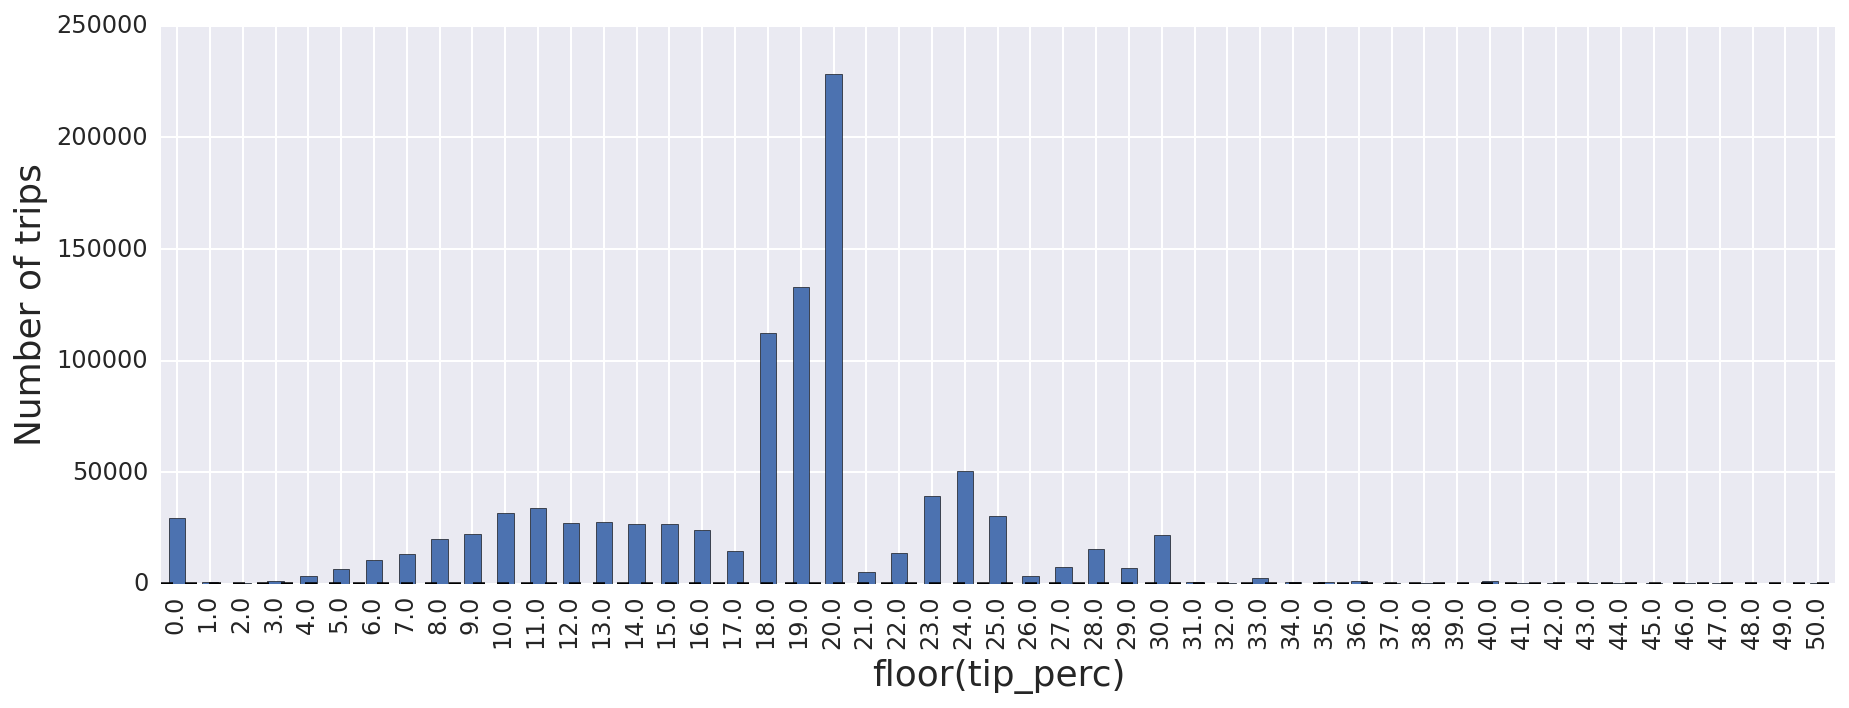
\includegraphics[width=140mm]{figures/ch_05/tip_perc.png}
  \caption{Representación del porcentaje de propinas redondeado a $0$ cifras decimales.}
  \label{fig:5.14}
\end{figure}

\pagebreak

Se observa que el valor más repetido es sin duda el $20\%$, que en realidad corresponde al rango $[20,\:21)$. Entonces, ¿se podría predecir qué propinas llegan como mínimo a esa \emph{normal social} y cuáles no? Para responder a esa pregunta, primero necesitamos transformar el atributo \emph{tip\_label} del dataset, para que este contenga tan sólo los valores ``$<\:20$'' y ``$>=\:20$'', los cuales se distribuyen por el dataset tal y como se muestra en la figura \ref{fig:5.15}.

\begin{figure}[H]
  \centering
  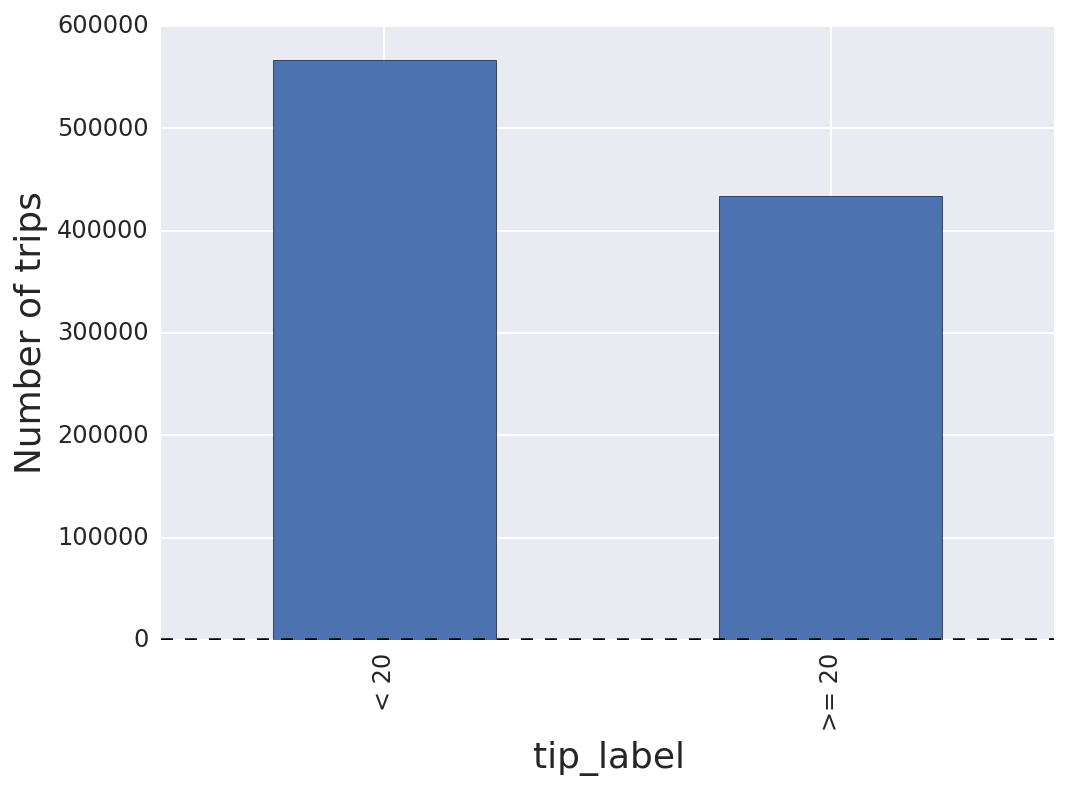
\includegraphics[width=100mm]{figures/ch_05/tip_label_2.png}
  \caption{Representación del nuevo atributo \emph{tip\_label}.}
  \label{fig:5.15}
\end{figure}

\begin{figure}[H]
  \centering
  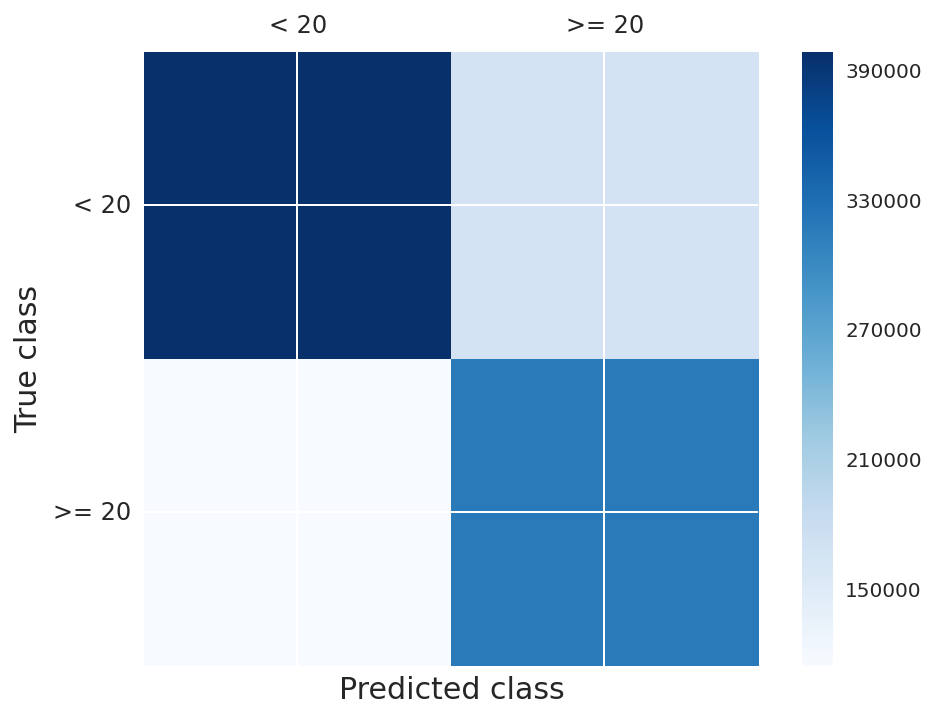
\includegraphics[width=100mm]{figures/ch_05/confusion_matrix_2.png}
  \caption{Matriz de confusión como resultado de la validación al clasificar las 2 nuevas clases de propinas.}
  \label{fig:5.16}
\end{figure}

Una vez hecho esto y ejecutado el algoritmo de aprendizaje con la misma configuración anterior, los resultados fueron muy distintos. $\mathbf{71.74\%}$ de exactitud, con la matriz de confusión de la figura \ref{fig:5.16}.

Para el \emph{área bajo las curvas} \emph{P/R} y \emph{ROC} (figuras \ref{fig:5.17} y \ref{fig:5.18}) también se obtuvieron resultados muy buenos, parecidos al de la exactitud. Para P/R, se tiene un \emph{área} de $0.78$ para la clase ``$<\:20$'', y de $0.68$ para ``$>=\:20$''. Si nos fijamos en ROC, el \emph{área} es de $0.75$ para ambas clases.

\begin{figure}[H]
  \centering
  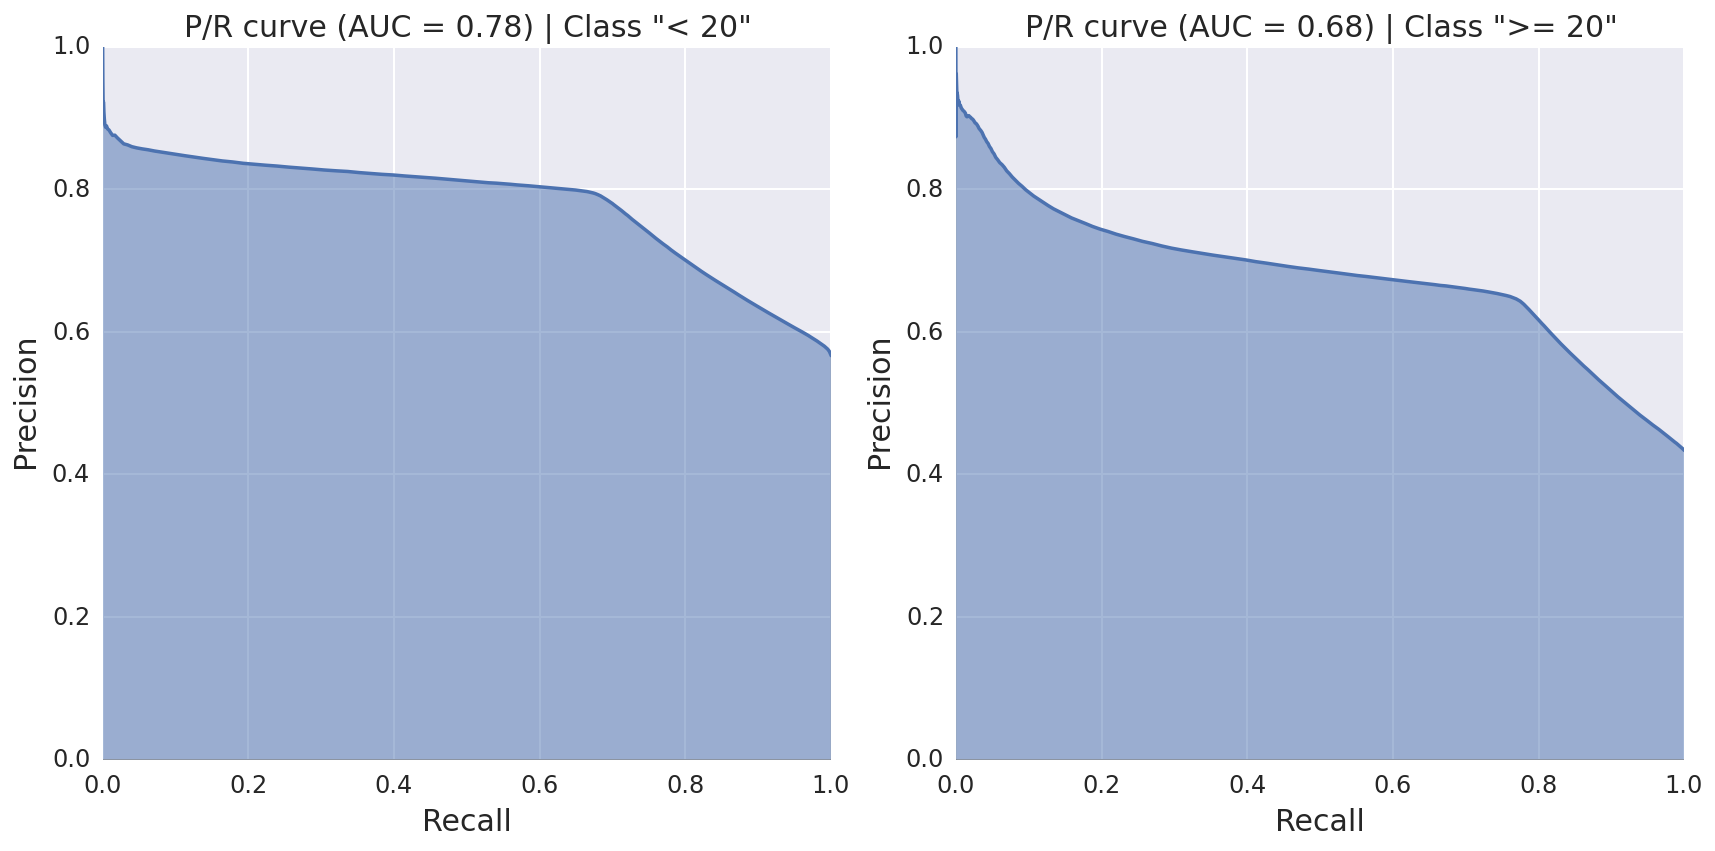
\includegraphics[width=140mm]{figures/ch_05/pr_auc.png}
  \caption{Área bajo la curva P/R del aprendizaje de las 2 clases de propinas.}
  \label{fig:5.17}
\end{figure}

\begin{figure}[H]
  \centering
  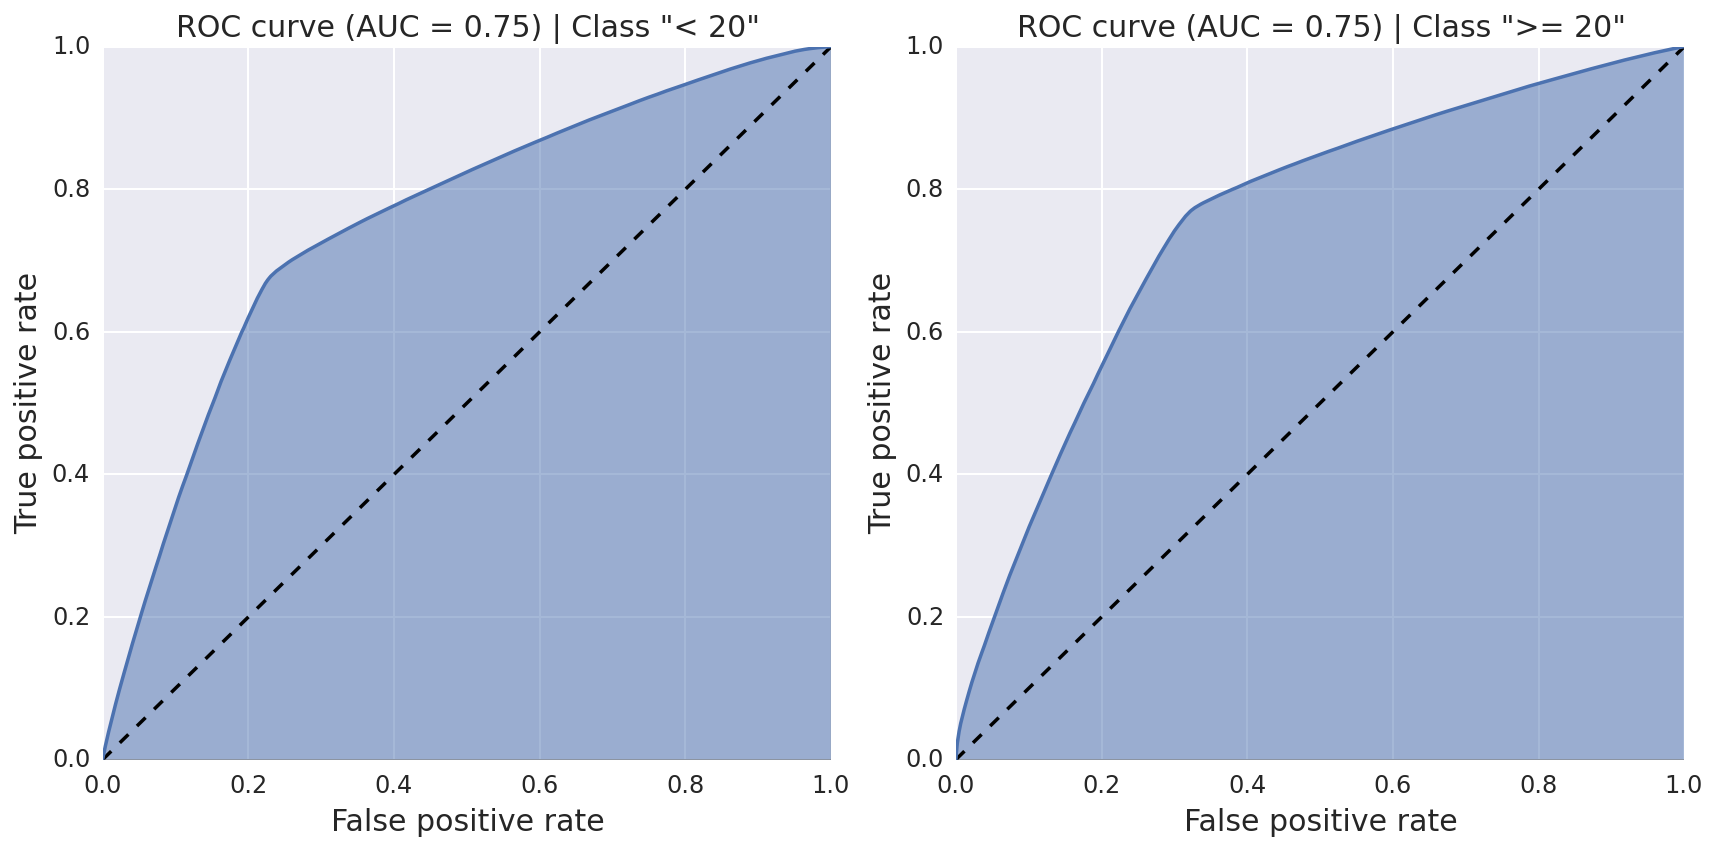
\includegraphics[width=140mm]{figures/ch_05/roc_auc.png}
  \caption{Área bajo la curva ROC del aprendizaje de las 2 clases de propinas.}
  \label{fig:5.18}
\end{figure}

Para finalizar con el aprendizaje, vamos a crear un pequeño ejemplo y ver cómo lo predice este random forest entrenado. Imaginemos que somos un broker que trabaja en la \emph{Bolsa de Nueva York}, \emph{New York Stock Exchange} en inglés, y que a las 11:30 sale del edificio para coger un tren en Penn Station con destino a Boston, para cerrar ciertos contratos con, por ejemplo, \emph{Boston Dynamics}\footnote{La famosa empresa de robótica: \url{http://www.bostondynamics.com/}}. Según Google Maps, el trayecto más corto son $4.4$ millas, en un total de 24 minutos. Para saber qué tarifa nos cobrarían, existen webs como \emph{TaxiFareFinder}\footnote{\url{http://www.taxifarefinder.com/}}, donde nos indica que este trayecto nos saldría por $16.30$ dólares.

¿Cuál sería la propina que daríamos al taxista? Teniendo en cuenta los datos anteriores, y sobre todo que somos brokers, se podría decir fácilmente que sería igual o supeiror al $20\%$. Y sin lugar a dudas, esta es la propina que el clasificador predice.

\section{Conclusiones} \label{sec:5.4}

Siendo los datos usados pertenecientes a un problema real, estando inicialmente en un estado para nada utilizable, y no procediendo de un ejercicio propuesto en algún medio, hacía que corriera el riesgo de no obtener ningún resultado. Teniendo esto en cuenta, hace que esté bastante contento con los resultados obtenidos, contando además que es la primera vez que me enfrento a un problema de semejante magnitud por mi cuenta.

Pero por supuesto, estos resultados son mejorables. Desde un punto de vista teórico, se podrían aplicar otras herramientas matemáticas para limpiar y crear nuevos atributos, y además se podría mejorar el aprendizaje afinando el modelo usado o utilizando otros algoritmos. Desde una perspectiva más práctica, unir este dataset con otros más podría generar uno mucho más potente. Desde la inclusión del estado meteorológico, a eventos deportivos y sus resultados, pasando por datos de los pasajeros, algo mucho más privado. Con esta información, el acierto casi total estaría asegurado, a costa de una posible fuga de privacidad. 

Por último, decir que el código generado para este caso práctico, en formato \emph{notebook} de IPython, está disponible en GitHub bajo \emph{licencia MIT}, como se comenta en el apéndice \ref{chap:ap_b}.
